\section{Materiales que contribuyen al examen}
\subsection{Tarea T2: My own Datacenter}
Descripción: Elegir (auto-inscribirse) en uno de los grupos DC para la entrega de esta actividad. (2 personas por grupo) no se admitirá personas trabajando solas.
Se pide diseñar un datacenter que cumpla con las siguientes caracteristicas:
\begin{itemize}
    \item Indicar una ubicación en Guayaquil donde pondria o implementaria un DC, y por qué?
    \item Que tipo de DC es viable implementar en esa zona (Tier 1, 2, 3, 4) y por qué?
    \item Es factible su diseño tenerlo en Green DC y por qué?
    \item Implementar su DC en CloudSIM con las siguientes características como mínimo (El grupo puede aumentar a su conveniencia su DC):
\end{itemize}
Two Datacenter whit 8 host per datacenter, Two Cores (1000 MIPS each core), 4 GB RAM, 100 GB Storage (100000 MB), 4000 Kbits/s bandwidth.

Cloudlets: 1500 cloudlets per datacenter with dynamic length (the user defines how many cloudlets for each datacenter), 20000+(random) instruction length, 400 kb output filesize, 1 core CPU requirement and Full Utilization.

Virtualization: 3 virtual machine, 50 GB storage disk, 2 GB Ram, 1 vCPU with 1000 MIPS, 2000 Kbits/s bandwidth and CloudleSchedulerTimeShared scheduler

Recursos:  CloudSimEx.java

Entregable: Screenshots del código y la (clase). (Evidencias de que lograron realizar el trabajo)y se seleccionarán de forma aleatoria 2 grupos para que presenten el diseño de su datacenter. 

Calificación: rúbrica.

\subsubsection{Evidencia y retoralimentación}
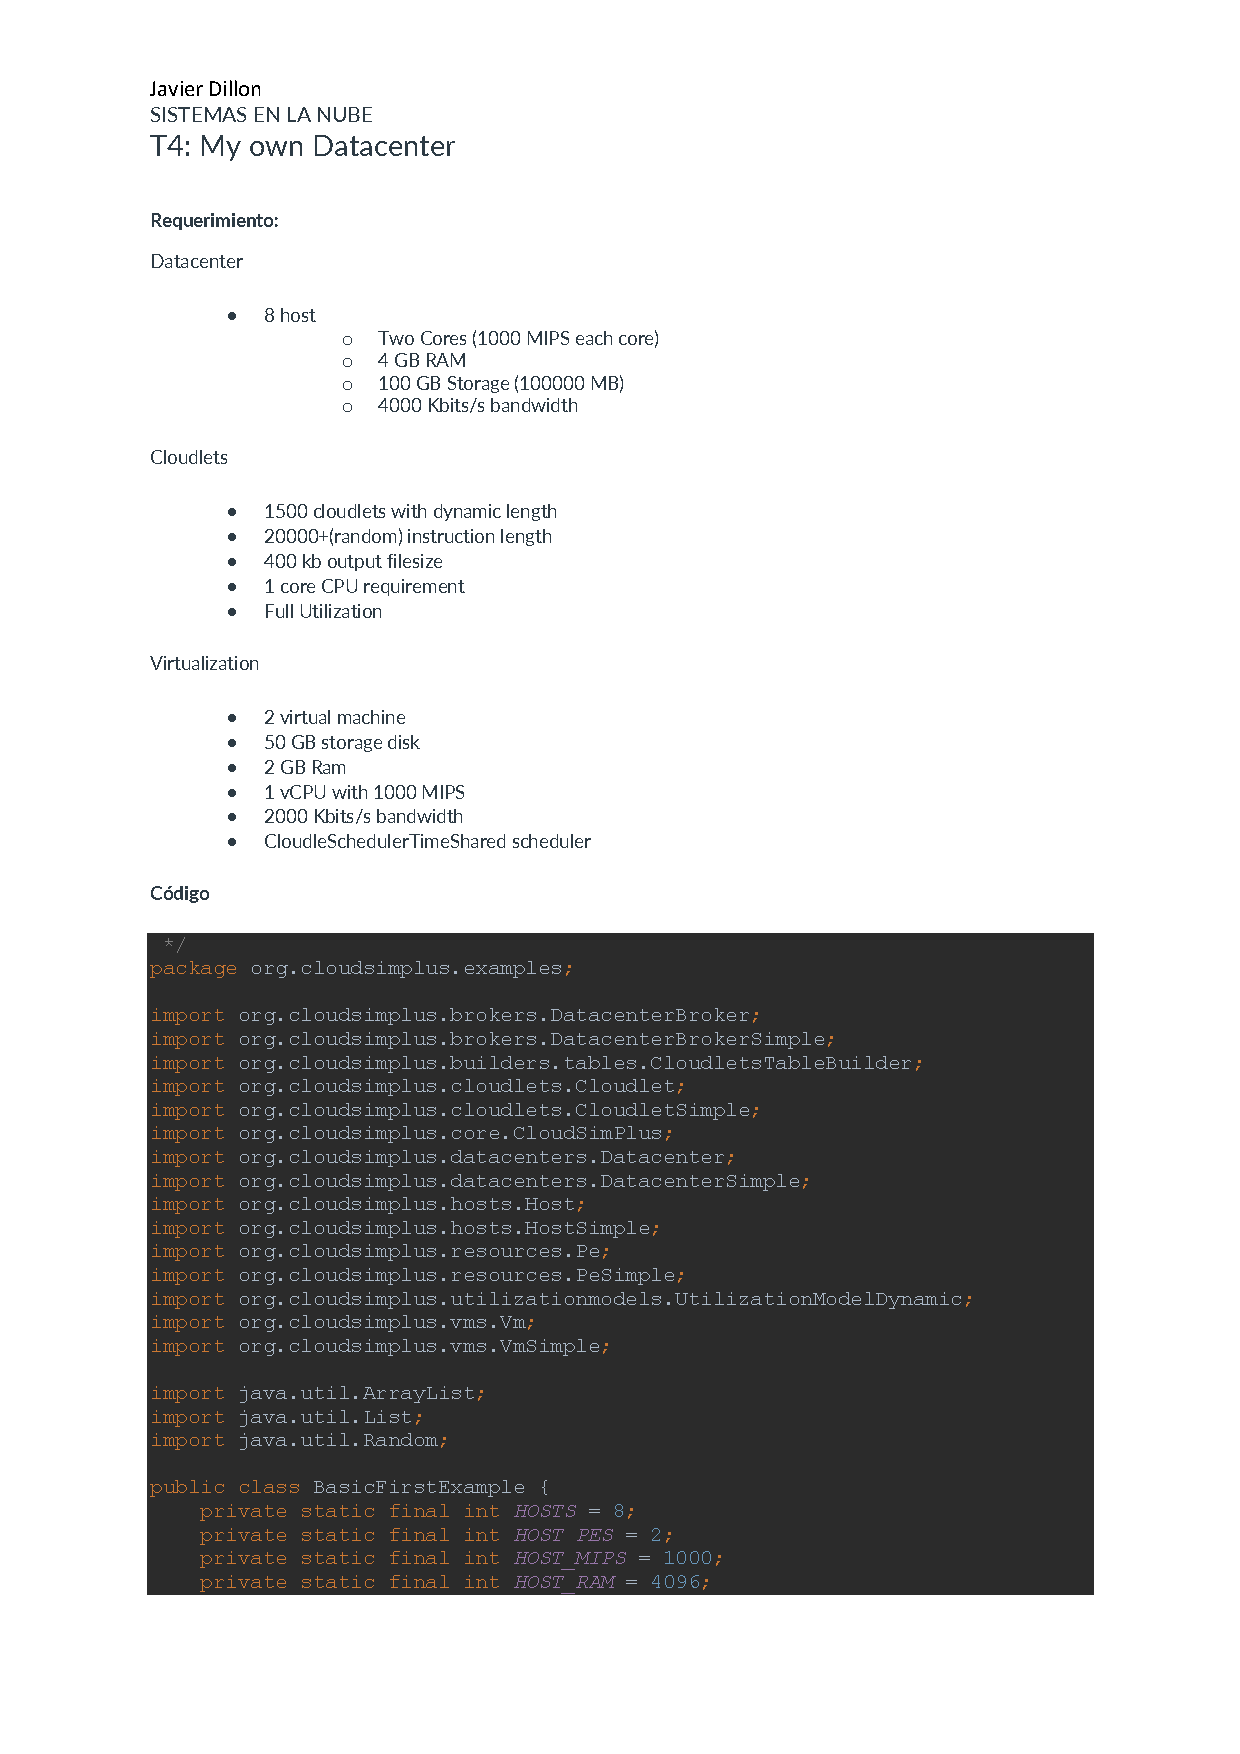
\includepdf[pages=-]{recursos/t2dat.pdf}

\begin{figure}[htbp]
    \centering
    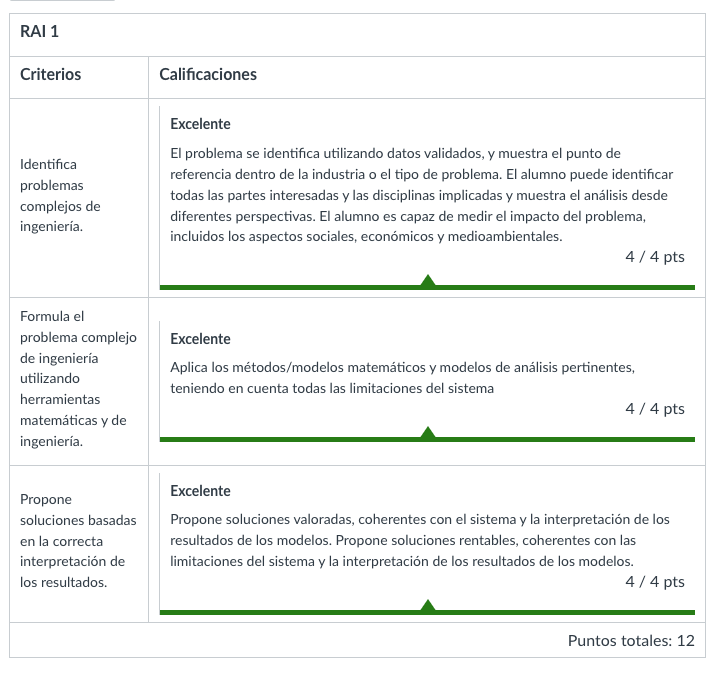
\includegraphics[width=\textwidth]{recursos/t2ru.png}
\end{figure}

\subsection{Tarea T3: SDN with MiniNet}
Instrucciones: El trabajo de emular una SDN es en grupo de 2. Se han creado grupos (sdn XX) donde pueden auto-registrarse (Quien no este en grupo - no se recibira la tarea). La descripción de la actividad la encuentran en el archivo  adjunto, sin embargo, dentro del archivo pueden encontrar información útil para el desarrollo de la actividad.

Recurso: AutonomousWork\_02.pdf

Entregable: Documento en formato tipo paper (Desarrollo - 3 pag. max.)  y el script de la red. El archivo debe contener las evidencias de que hubo conectividad en toda la red. 

Calificación: Rúbrica. 

\subsubsection{Evidencia y retroalimentación}

\begin{figure}[htbp]
    \centering
    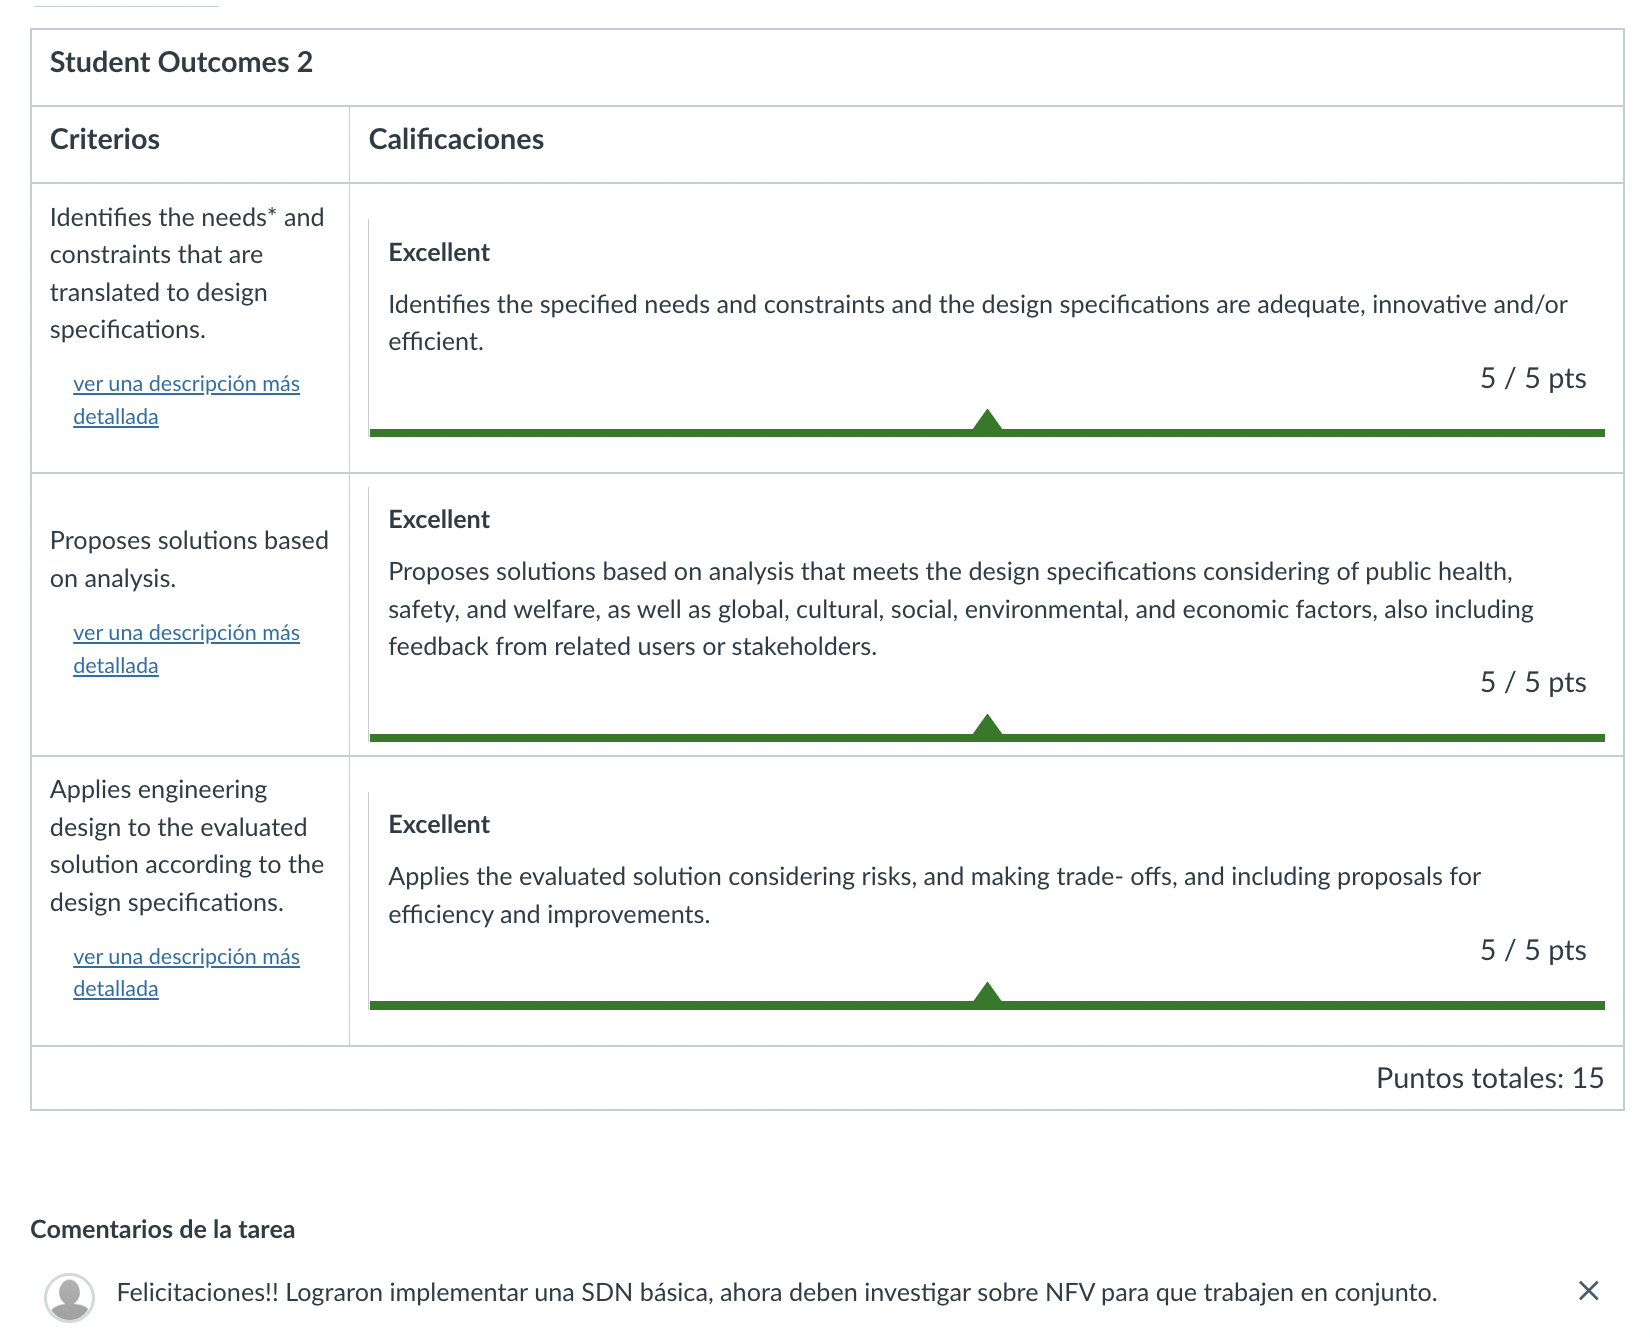
\includegraphics[width=\textwidth]{recursos/sdn_ru.png}
\end{figure}

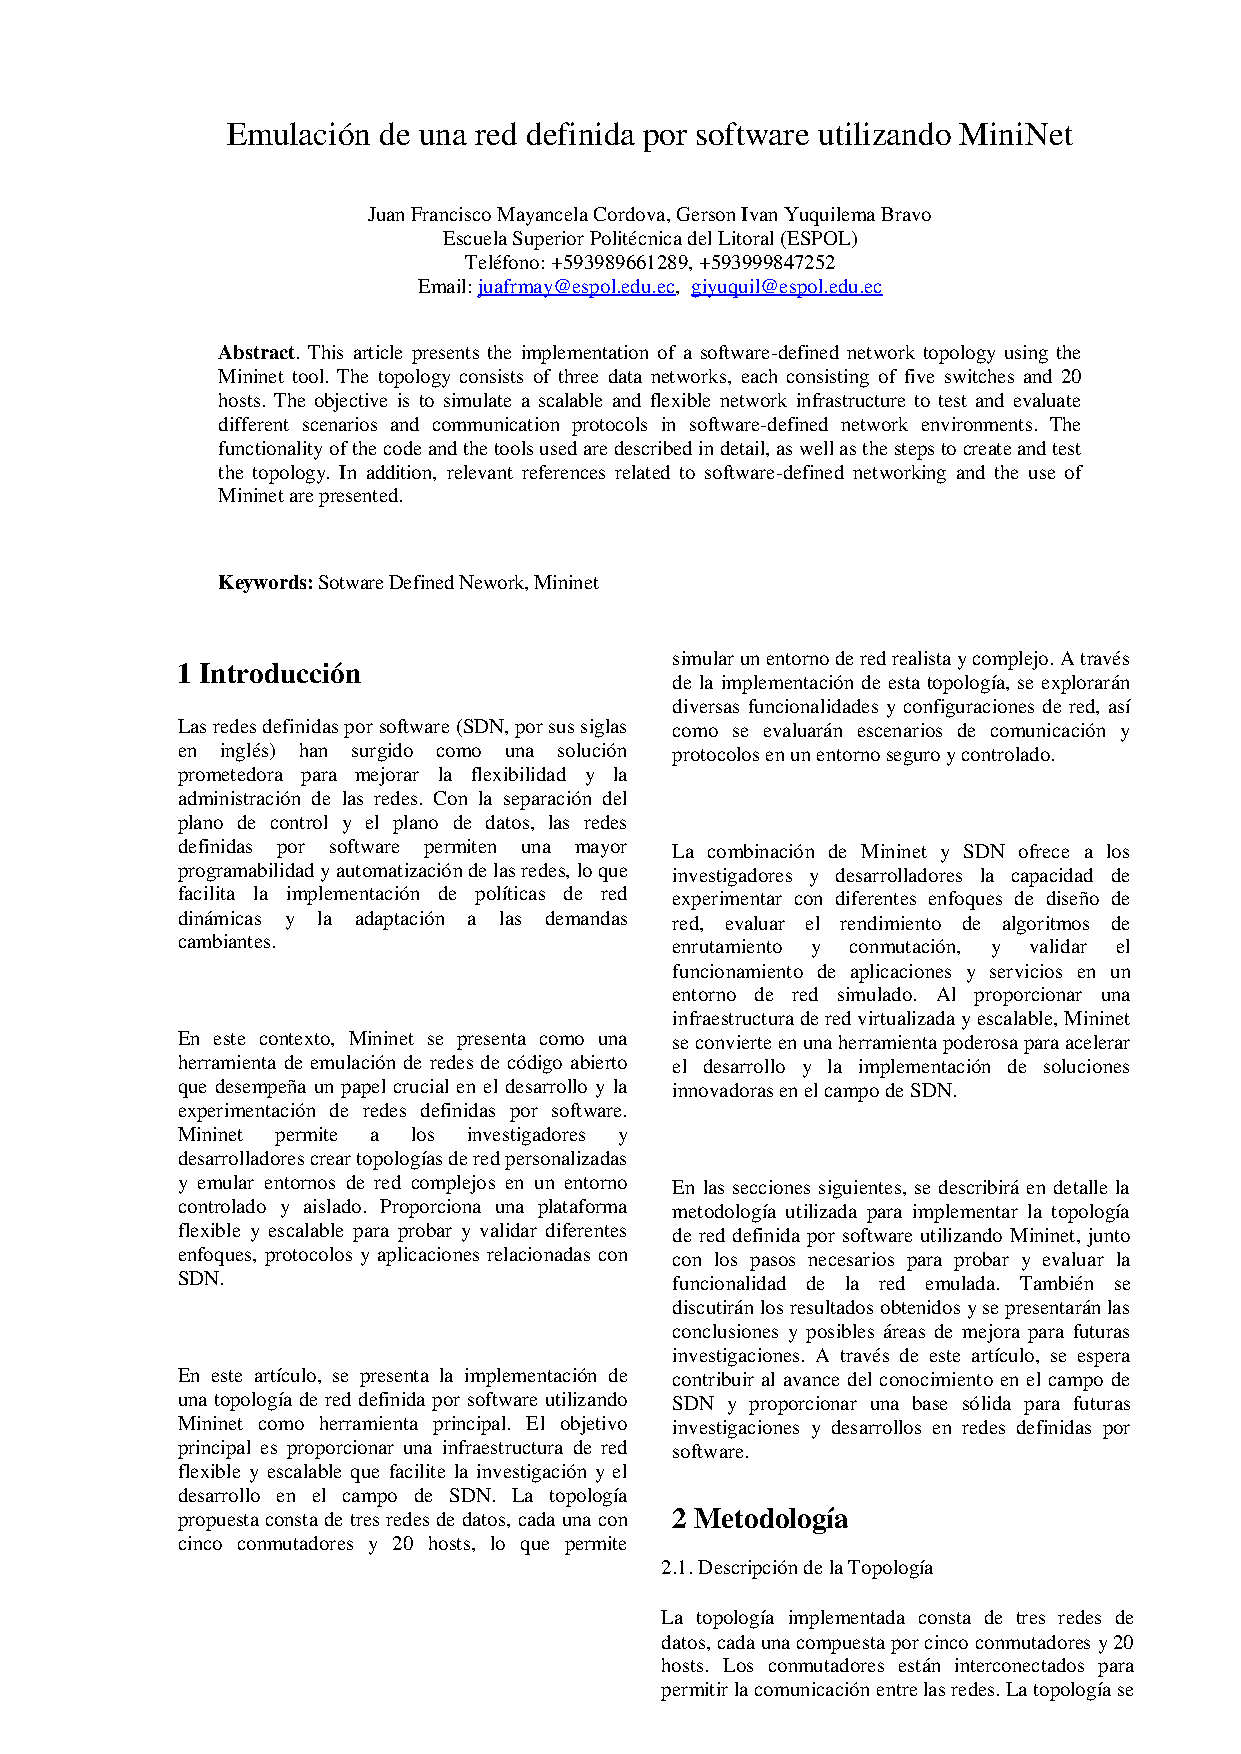
\includepdf[pages=-]{recursos/sdnt3.pdf}

\subsection{Examen de primera evaluación}
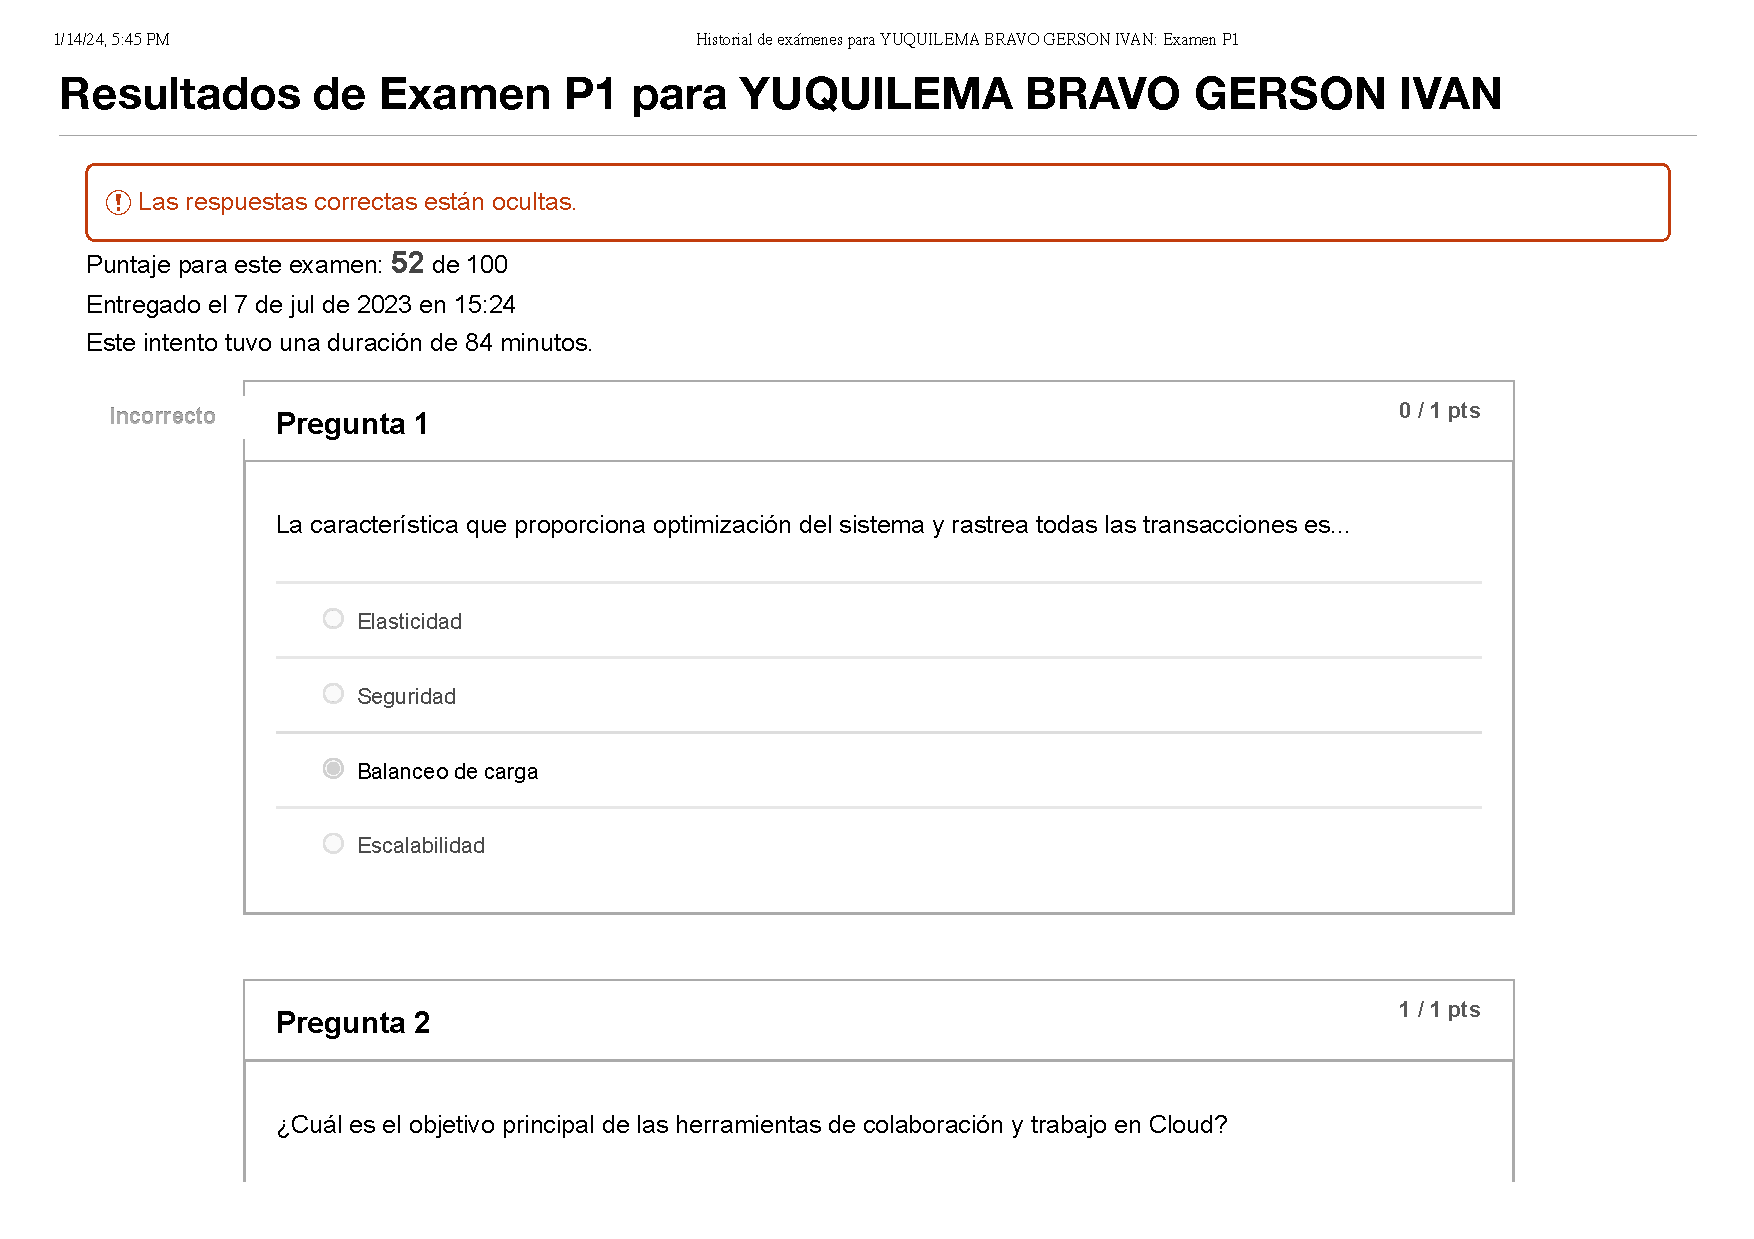
\includepdf[pages=-]{recursos/exa/exp1.pdf}

\subsection{Examen de segunda evaluación}
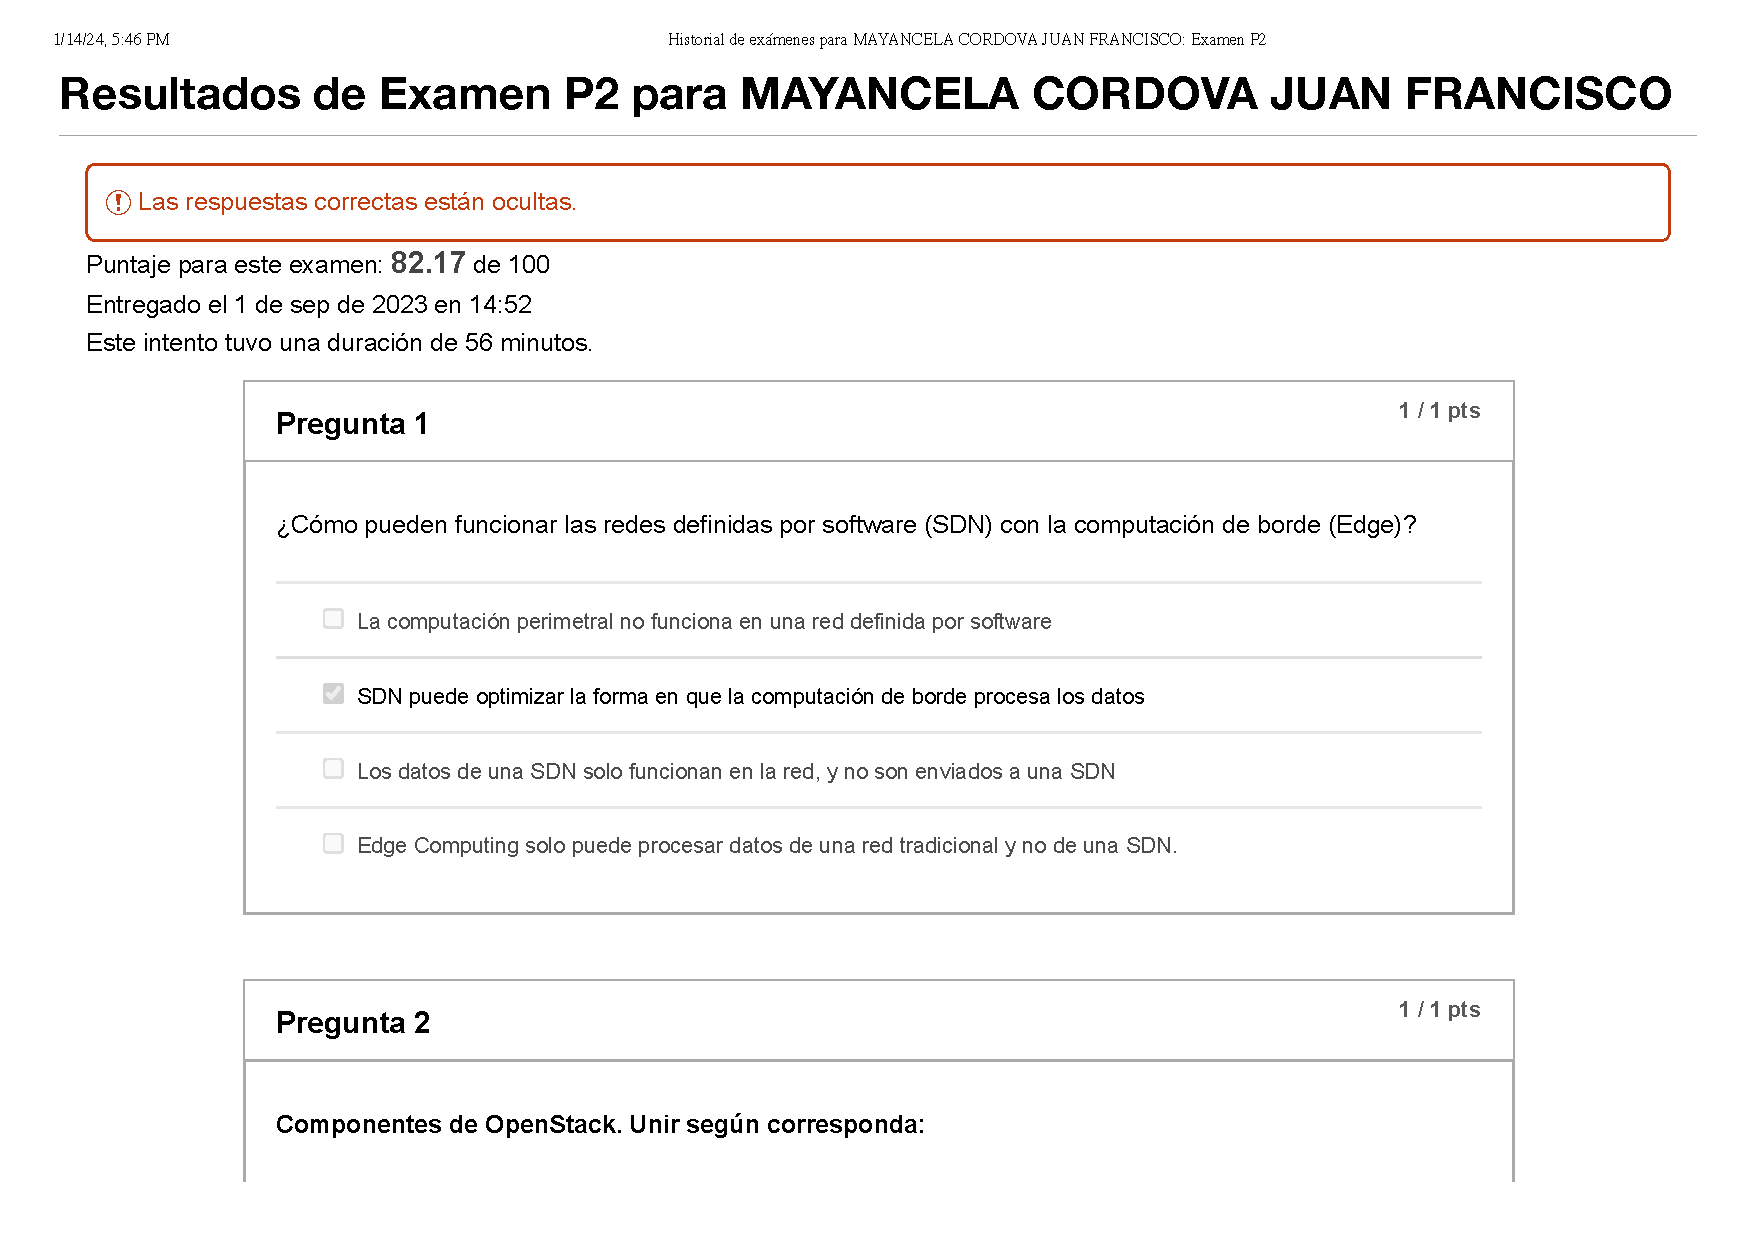
\includepdf[pages=-]{recursos/exa/exp2.pdf}